% /Users/astrand/src/kernelPop/kernelPop-intro/kernelPop-intro.tex
% $Modified:  Mon Oct 23 23:39:53 EDT 2006$


\documentclass[10pt]{article}

\usepackage{color}
\usepackage{fullpage}
\usepackage{natbib}
\usepackage{graphicx}
\usepackage{times}
\usepackage{Sweave}
\usepackage{array}
%\usepackage{babel}

\newcommand{\KP}{\texttt{kernelPop}}
\newcommand{\code}[1]{\texttt{#1}}
\title{KernelPop}
\author{Allan Strand\\[14pt] Department of Biology\\College of
  Charleston\\Charleston, SC 29424\\stranda@cofc.edu}
\begin{document}
%\VignetteIndexEntry{KernelPop}

\maketitle


\section{Introduction}
\label{sec:introduction}
\KP is a software environment for simulating population genetics in a
explicitly spatial manner.  It is a discrete-time and
individual-based.  This software provides flexibility at several
levels of organization.  From general to narrow these include:
Landscapes, habitats, populations, individuals, and loci.  \KP
implements this structure for a single species using a single
list-based data structure in R.  The vast majority of functions either
help create or modify this structure or to extract information from
it.  

Using the set of tools provided with KernelPop along with R, it is
possible to define and execute almost any demographic scenario that
can be implemented in discrete-time.  The actual simulations are
carried out in C++ to increase speed.

\subsection{Comparison to other software}
At least two other packages offer a generic simulation environment for
neutral population genetics, \texttt{EASYPOP} and \texttt{Rmetasim}.
Table~\ref{tab:comp} summarizes these differences. In
short,\texttt{EASYPOP} is faster and simpler to use, but does not
include as much ecological realism as \texttt{kernelPop}.

% latex table generated in R 2.5.0 by xtable 1.4-3 package
% Sun Feb 25 22:23:14 2007
\begin{table}[p]

  \caption{Comparison between three individual-based simulators for population genetics. 
    $^\dag$These features are implemented through the demographic matrix parameterization of 
    Rmetasim and kernelPop. $^\S$There are many R packages designed to estimate population 
    genetic parameters including: ape, ade4, genetics, geneland, and hierfst. Because both 
    Rmetasim and kernelPop can be simulated a generation at a time, it is possible to 
    create quite elaborate selection schemes using R-code modifications of landscape objects
  }


\begin{center}
\hspace*{-0.25in}
\begin{tabular}{p{1.3in}|p{1.68in}p{1.68in}p{1.68in}}
  \hline
 & EASYPOP & Rmetasim & kernelPop \\ \hline
  \hline
Within-population demography & Zygote-Adult & Stage- or age-based, overlapping generations & Stage- or age-based, overlapping generations \\  \hline
  Population structure & patchy & patchy & patchy or continuous \\  \hline
  Patch quality & constant & variable & variable \\  \hline
  Dispersal kernels & among populations, exponential & among populations\dag & among and within populations, determined by choices among several PDFs \\  \hline
  Classical dispersal models & island, stepping-stone & island, stepping stone, migration matrix & island, stepping-stone, migration matrix combined with cell above \\  \hline
  Dispersal Stage & zygote & male gametes and/or any diploid life-stage & male gametes and/or any diploid life-stage \\  \hline
  Dispersal parameters  & vary among populations & vary among individual demographic stages and populations & vary among individual demographic stages and populations \\  \hline
  Metapopulation parameters & constant, equal, population sizes  & Density-dependent or hard carrying capacity varies among patches; extinction rate varies among patches & Density-dependent or hard carrying capacity varies among patches; extinction rate varies among patches \\  \hline
  Genealogy & Complete retrievable & Single-generation & Single-generation \\  \hline
  Mating systems & selfing, random, monogamy, polygyny & selfing,random, monogamy\dag, polygyny\dag & selfing,random, monogamy\dag, polygyny\dag \\  \hline
  Sexuality & haploid, haplodiploid, hermaphrodite, dioecious & hermaphrodite, dioecious\dag & hermaphrodite, dioecious\dag \\  \hline
  Clonal reproduction & yes & no & no \\  \hline
  Recombination  & variable recombination for diploid loci, recombination possible among haploid loci & unlinked diploid loci, no recombination among haploid loci & unlinked diploid loci, no recombination among haploid loci \\  \hline
  Mutation models & Strict stepwise, k-allele, mixtures between stepwise and k-allele, mixtures between two stepwise & Strict stepwise, infinte allele, k-allele, sequence & Strict stepwise, infinte allele, k-allele, sequence \\  \hline
  Selection & no & Can be implemented in R & Can be implemented in R \\  \hline
  Output formats & Arlequin, GenPop FSTAT & Arlequin, GenePop, GDA, migrate, R\S & Arlequin, GenePop, GDA, migrate, fdist, R\S \\  \hline
  Numbers of parameters & lower & moderate & higher \\  \hline
   \hline
\end{tabular}
\end{center}
\label{tab:comp}
\end{table}

\section{Landscape object}
\label{sec:landscape-object}


\begin{figure}
  \centering
  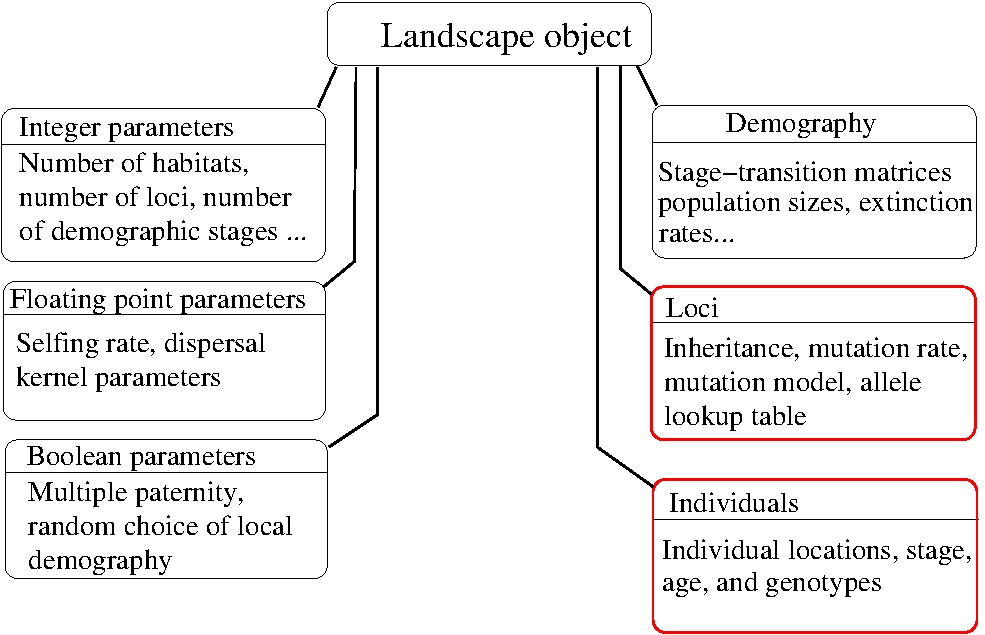
\includegraphics{landscape-object}
  \caption{Schematic of the high-level organization of the landscape object}
  \label{sec:landscape-object-fig}
\end{figure}


Figure \ref{sec:landscape-object-fig} illustrates the high-level
organization of a landscape object.  The following subsections will
document the different sub-components.

Each will:
\begin{itemize}
\item describe the sub-object
\item describe the function(s) used to create it
\end{itemize}

The first step in creating a landscape object is to create a skeleton landscape
\begin{Schunk}
\begin{Sinput}
> land <- landscape.new.empty()
> names(land)
\end{Sinput}
\begin{Soutput}
[1] "intparam"    "switchparam" "floatparam"  "demography"  "loci"       
[6] "expression"  "individuals"
\end{Soutput}
\end{Schunk}

\subsection{intparam}
\label{sec:intparam}

The \code{intparam} element of the landscape object describes integer values, they include:
\begin{description}

\item [habitats (h)] This parameter provides the number of rectangular
habitats within a landscape.  These habitats may or may not be
populated.

\item [stages (s)] The number of demographic stages present in a single habitat.

\item [locusnum] The number of genetic loci to be simulated (not changeable directly)

\item [numepochs ] It is possible to have multiple epochs during the
  course of a simulation.  This can be implemented either in R by the
  investigator (recommended) or in C++ by specifying multiple epochs
  sub-objects.  numepochs specifies the number of these to be used in
  C++.  (not changeable directly)

\item [currentgen (cg)] Current generation (year) of a simulation (best to leave unchanged)

\item [currentepoch (ce)] Current epoch (leave unchanged)

\item [totalgens (totgen)] Total number of generations that can be simulated

\item [numdemos] The number of different within-habitat demographies.
  These can vary across a landscape. (not changeable directly)

\item [maxlandsize (maxland)] Total number of individuals that can be simulated

\item [nphen (np)] not used yet.

\end{description}

The \code{args()} provides the default values for this
function\footnote{All code in this document should be available in
  annotated form in the file kernelPop-intro.R distributed with this pdf.
  If you source it into R it will execute the code and produce similar
  results.  If you set '\code{par(ask=T)}' before '\code{sourcing}',
  the graphs (and subsequent steps!) will wait for you to hit return}.

\begin{Schunk}
\begin{Sinput}
> args(landscape.new.intparam)
\end{Sinput}
\begin{Soutput}
function (rland, h = 1, s = 1, cg = 0, ce = 0, totgen = 1000, 
    maxland = 2e+05, np = 0) 
NULL
\end{Soutput}
\begin{Sinput}
> land <- landscape.new.intparam(land, h = 4, s = 6)
\end{Sinput}
\end{Schunk}

Note that this function takes a landscape object (in this case,
skeleton) as one of its parameters.  It returns the modified
landscape.  This is typical for the landscape creation and
modification functions

\subsection{floatparams}
\label{sec:floatparams}
These are parameters describe selfing rate (s) and then a set of
dispersal characteristics that will apply to all stages in the
simulation
\begin{description}
\item [selfing (s)] Selfing rate in a mixed-mating model
\item [seedmu ] Scale of first seed dispersal distribution
\item [seedshape ] Shape of first seed dispersal distribution
\item [ pollenmu] Scale of first pollen dispersal distribution
\item [pollenshape] Shape of first pollen dispersal distribution
\item [seedmu2] Scale of second seed dispersal distribution
\item [seedshape2] Shape of second seed dispersal distribution
\item [seedmix] mixture parameter between the two seed distributions (1=all dist 1, 0=all dist 2)
\item [aspect] Factor that reduces the y-dimension of dispersal. A
  value of 1 is equal x and y dispersal.  This does not change the
  dispersal distances, however, just their direction
\item [pollenmu2] Scale of second pollen dispersal distribution
\item [pollenshape2] Shape of second pollen dispersal distribution
\item [pollenmix] mixture parameter between the two pollen distributions (1=all dist 1, 0=all dist 2)
\end{description}

\begin{Schunk}
\begin{Sinput}
> args(landscape.new.floatparam)
\end{Sinput}
\begin{Soutput}
function (rland, s = 0, seedscale = c(10, 10), seedshape = c(10, 
    10), seedmix = 1, pollenscale = c(2, 10), pollenshape = c(2, 
    6), pollenmix = 1, asp = 1, mindens = 1e-25) 
NULL
\end{Soutput}
\begin{Sinput}
> land <- landscape.new.floatparam(land)
\end{Sinput}
\end{Schunk}

\subsection{switchparam}
\label{sec:switchparams}
These are boolean parameters that make choices about a landscape
\begin{description}

\item [randepoch] If 0, choose different epochs in the order they are specified.  If 1 choose epochs at random (again multiple epochs are kind of obsolete, but are built into the basic C++ engine) (don't change)
\item [randdemo] If there are multiple local demographies for
  different habitats, choose among them at random for each habitat if
  1; if 0, assign them in the same order as the habitats are defined.
\item [multp] If 1 each zygote potentially has a different father
  (slower).  If 0 all offspring for a mother in a particular year are
  full-sibs
\end{description}

\begin{Schunk}
\begin{Sinput}
> args(landscape.new.switchparam)
\end{Sinput}
\begin{Soutput}
function (rland, re = 0, rd = 0, mp = 1) 
NULL
\end{Soutput}
\begin{Sinput}
> land <- landscape.new.switchparam(land)
\end{Sinput}
\end{Schunk}

\subsection{demography}
\label{sec:demography}

This sub-object basically defines all of the vital rates that determine
survival and reproduction.  It also contains functions that define
metapopulation characteristics like extinction rate per habitat,
carrying capacity per habitat and dispersal parameters.

It is divided into two subcomponents, each of which is further
divided.

\subsubsection{localdem}
\label{sec:localdem}
This is a description of the sub-matrices that define demography in
each habitat.  It is a list of any length between 1 and the number of
habitats.  Depending on the value of \code{randdemo} in the switch
subcomponent, each habitat is either: 1) randomly assigned an element
from this list with probabilities that can be defined in the epochs
sub object (sec. \ref{sec:epochs}) or 2) assigned demographies by
cycling through this list.

Each element is composed of three matrices that describe a stage based
demography. Figure

\begin{figure}
  \centering
  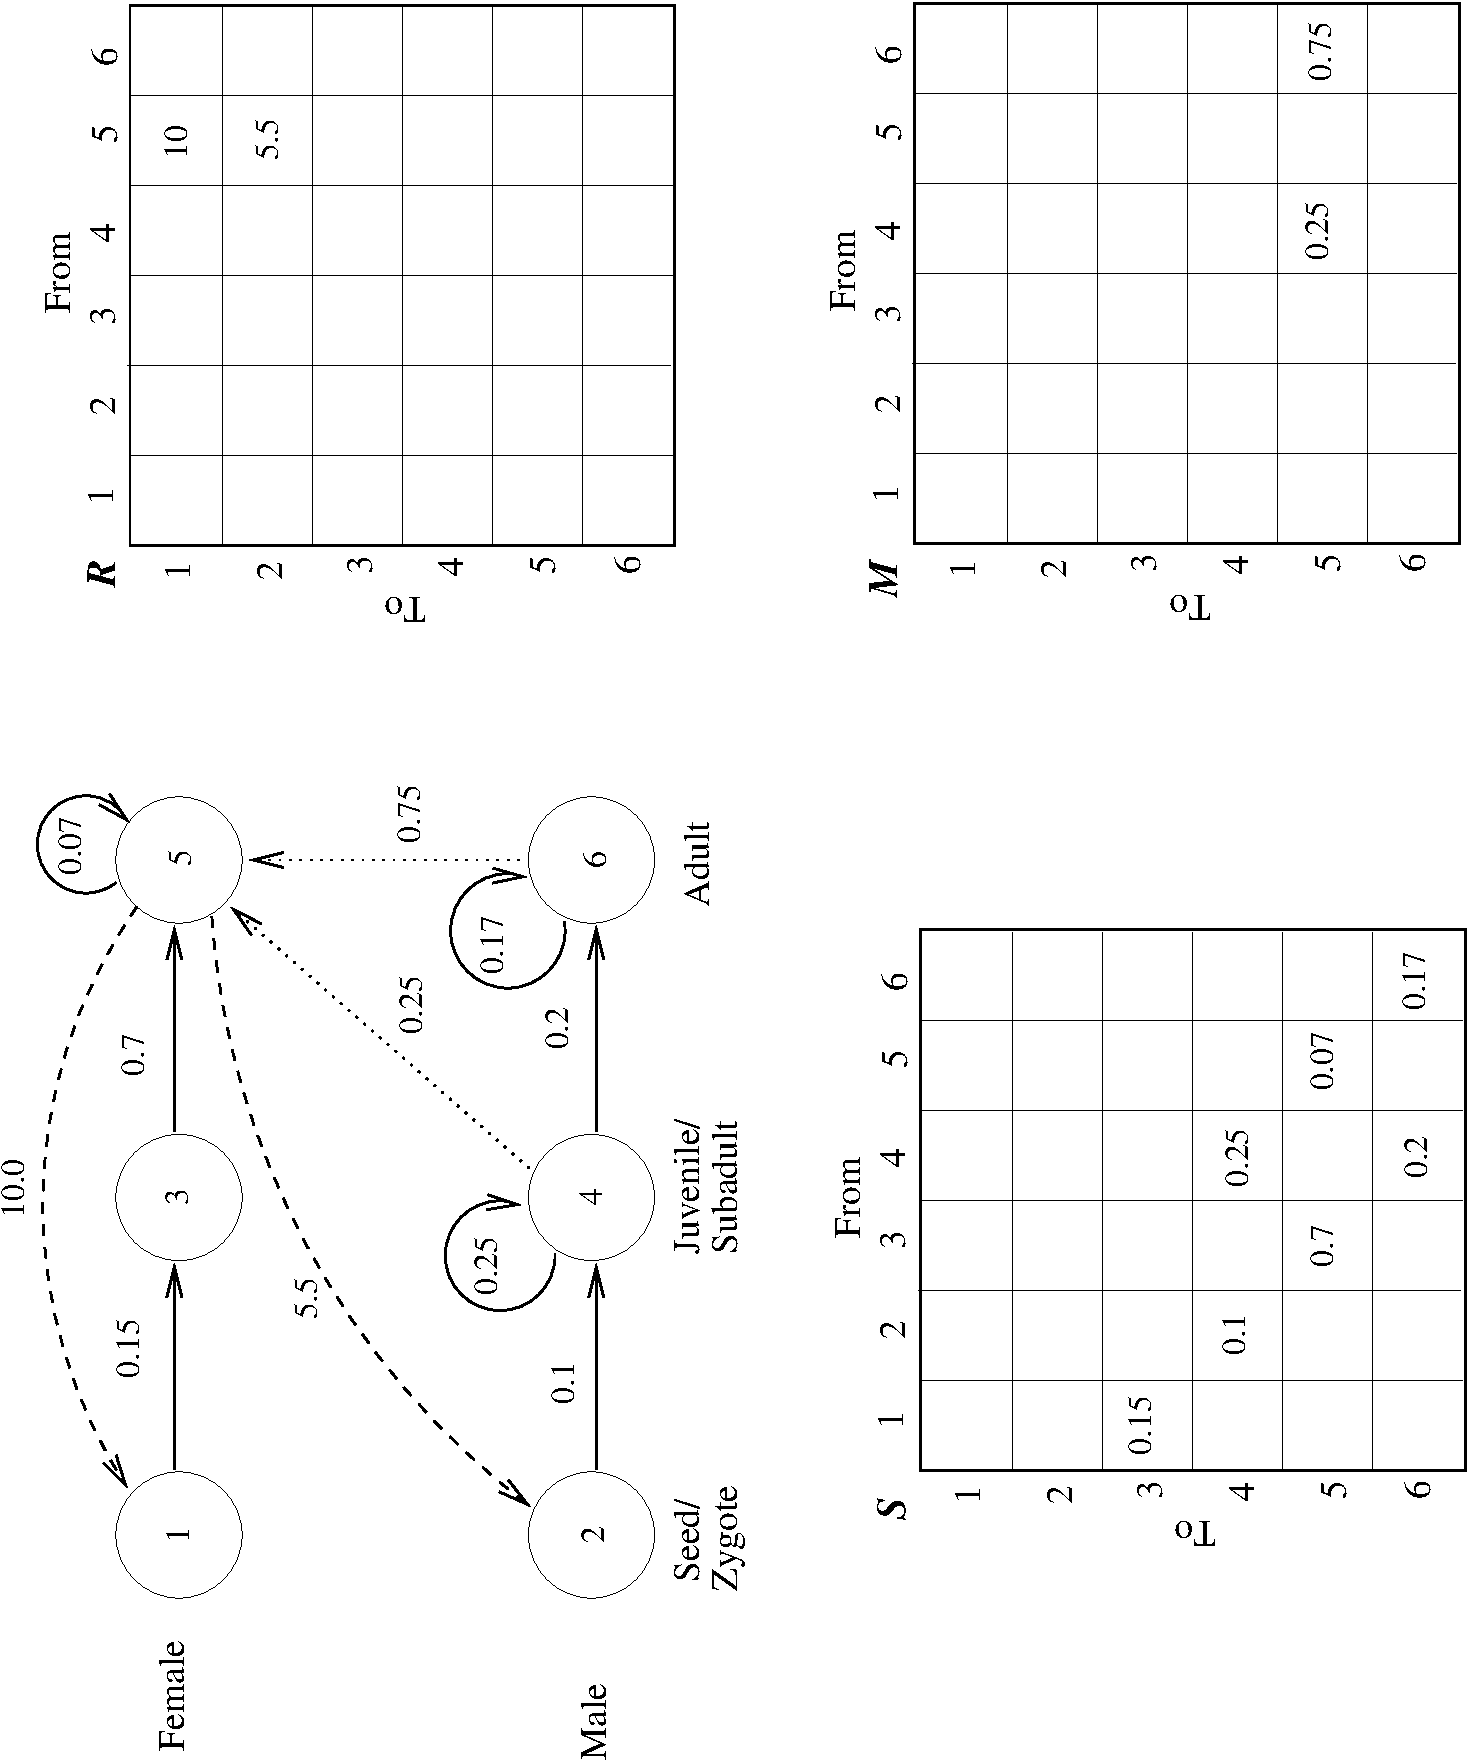
\includegraphics[angle=270]{demography.pdf}
  \caption{ Stage-based demography within habitats.  This life-cycle
    has six stages, essentially three male and three female stages.
    The rates of male and female survival are different (for example,
    intermediate sized females (stage 3) have high probabilities of
    growing into adults in the next season).  Females produce a mean of
    10 and 5.5 male and female juveniles per generation, respectively.
    These are means of Poisson distributions.  Both stage 4 and stage
    5 can produce pollen though stage 6 produces three times the
    pollen on average.}
  \label{fig:demogr}
\end{figure}
\begin{Schunk}
\begin{Sinput}
> S <- matrix(c(0, 0, 0, 0, 0, 0, 0, 0, 0, 0, 0, 0, 0.18, 0, 0, 
+     0, 0, 0, 0, 0.14, 0, 0.26, 0, 0, 0, 0, 0.7, 0, 0.09, 0, 0, 
+     0, 0, 0.2, 0, 0.18), byrow = T, nrow = 6)
> R <- matrix(c(0, 0, 0, 0, 14, 0, 0, 0, 0, 0, 8.5, 0, 0, 0, 0, 
+     0, 0, 0, 0, 0, 0, 0, 0, 0, 0, 0, 0, 0, 0, 0, 0, 0, 0, 0, 
+     0, 0), byrow = T, nrow = 6)
> M <- matrix(c(0, 0, 0, 0, 0, 0, 0, 0, 0, 0, 0, 0, 0, 0, 0, 0, 
+     0, 0, 0, 0, 0, 0, 0, 0, 0, 0, 0, 0.25, 0, 0.75, 0, 0, 0, 
+     0, 0, 0), byrow = T, nrow = 6)
> args(landscape.new.local.demo)
\end{Sinput}
\begin{Soutput}
function (rland, S, R, M) 
NULL
\end{Soutput}
\begin{Sinput}
> land <- landscape.new.local.demo(land, S, R, M)
> print("add a new local demography with different Reproduction")
\end{Sinput}
\begin{Soutput}
[1] "add a new local demography with different Reproduction"
\end{Soutput}
\begin{Sinput}
> R2 <- matrix(c(0, 0, 0, 0, 8, 0, 0, 0, 0, 0, 5.5, 0, 0, 0, 0, 
+     0, 0, 0, 0, 0, 0, 0, 0, 0, 0, 0, 0, 0, 0, 0, 0, 0, 0, 0, 
+     0, 0), byrow = T, nrow = 6)
> land <- landscape.new.local.demo(land, S, R2, M)
\end{Sinput}
\end{Schunk}

The previous code block installed two local demographies into the localdem list.

\subsubsection{epochs}
\label{sec:epochs}
This is a list of elements each of which define landscape-level
characteristics.  Currently my recommendation is to declare only 1 and
modify it in R to change simulations through time.

\paragraph{Landscape demographic characteristics}
\label{sec:landc-demogr-char}

The matrices defined in section \ref{sec:localdem} comprise
sub-matrices of 3 larger matrices that are (number of habitats)*(number
of stages) in dimension This is similar to a multi regional model.
Figure may help illustrate this concept, though it has the
reproduction and survival matrices summed into a single matrix.  
\begin{figure}
  \centering
  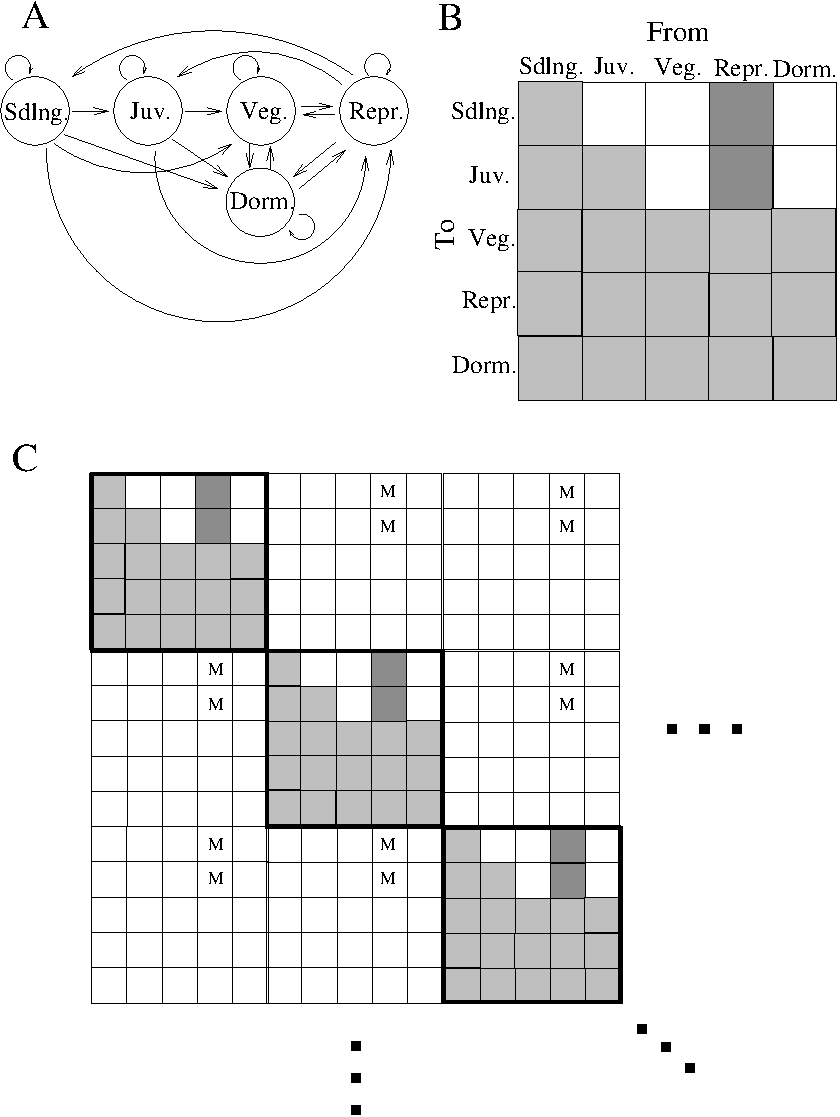
\includegraphics{metamarkov.pdf}
  \caption{Schematic of landscape matrix metaphor}
  \label{fig:landmat}
\end{figure}

These matrices can implement dispersal among populations independent
of the dispersal kernels defined in the next paragraphs.  I wanted to
maintain this ability because it provides a convenientt way to model
management efforts like transplants, introductions, and stocking efforts.

For most uses of \KP, these matrices can be set to zero in each cell.
They still need to be defined, however.  The matrix \code{zeromat}
will be used for each of the three landscape matrices

\begin{Schunk}
\begin{Sinput}
> zeromat <- matrix(0, nrow = 4 * 6, ncol = 4 * 6)
\end{Sinput}
\end{Schunk}

\paragraph{Vectors describing habitats within a landscape}
\label{Probabilities}
Vectors with length equal to the number of habitats are defined in this sub-element to characterize:
\begin{description}
\item[extinction] the yearly rate of extinction of each habitat
\item[carrying capacity] the largest number of individuals supported in each habitat 
\end{description}
\begin{Schunk}
\begin{Sinput}
> extnct <- c(0, 0.1, 0, 0.1)
> k <- c(1000, 600, 600, 1000)
\end{Sinput}
\end{Schunk}

Vectors with length equal to the length of the local demography
describe the probability of picking a local demography from the
localdem list.  Always defined, but only used if \code{randdemo}
(section~\ref{sec:switchparams}) is set appropriately.
\begin{Schunk}
\begin{Sinput}
> ldem <- c(0.5, 0.5)
\end{Sinput}
\end{Schunk}

\paragraph{Seed dispersal kernel matrix}
This is a matrix that has (number of habitats)*(number of stages) rows
and six columns.  If not specified, a working matrix is constructed
from the floatparam elements

The rows correspond to stages in the landscape.  The columns correspond to (in order)
\begin{enumerate}
\item the seed dispersal kernel.  This can be 1,2, or 3 (the default).
  1 and 2 are really just special cases of the mixed pdf (kernel 3)
\item the scale parameter for kernel component 1
\item the shape parameter for kernel component 1
\item the scale parameter for kernel component 2
\item the shape parameter for kernel component 2
\item the mixing parameter.  Ranges from 0 to 1.  If 1 dispersal is
  determined solely by kernel 1.  If 0, dispersal is determined solely
  by kernel 2.  Intermediate values represent a mixture.
\end{enumerate}
\begin{Schunk}
\begin{Sinput}
> sk <- matrix(0, nrow = 4 * 6, ncol = 6)
> sk[, 1] <- rep(3, 4 * 6)
> sk[, 2] <- rep(10, 4 * 6)
> sk[, 3] <- rep(1.1, 4 * 6)
> sk[, 4] <- rep(100, 4 * 6)
> sk[, 5] <- rep(50, 4 * 6)
> sk[, 6] <- rep(0.5, 4 * 6)
> sk
\end{Sinput}
\begin{Soutput}
      [,1] [,2] [,3] [,4] [,5] [,6]
 [1,]    3   10  1.1  100   50  0.5
 [2,]    3   10  1.1  100   50  0.5
 [3,]    3   10  1.1  100   50  0.5
 [4,]    3   10  1.1  100   50  0.5
 [5,]    3   10  1.1  100   50  0.5
 [6,]    3   10  1.1  100   50  0.5
 [7,]    3   10  1.1  100   50  0.5
 [8,]    3   10  1.1  100   50  0.5
 [9,]    3   10  1.1  100   50  0.5
[10,]    3   10  1.1  100   50  0.5
[11,]    3   10  1.1  100   50  0.5
[12,]    3   10  1.1  100   50  0.5
[13,]    3   10  1.1  100   50  0.5
[14,]    3   10  1.1  100   50  0.5
[15,]    3   10  1.1  100   50  0.5
[16,]    3   10  1.1  100   50  0.5
[17,]    3   10  1.1  100   50  0.5
[18,]    3   10  1.1  100   50  0.5
[19,]    3   10  1.1  100   50  0.5
[20,]    3   10  1.1  100   50  0.5
[21,]    3   10  1.1  100   50  0.5
[22,]    3   10  1.1  100   50  0.5
[23,]    3   10  1.1  100   50  0.5
[24,]    3   10  1.1  100   50  0.5
\end{Soutput}
\end{Schunk}

\paragraph{Pollen dispersal kernel matrix}
This is a matrix that has (number of habitats)*(number of stages) rows
and six columns.  If not specified, a working matrix is constructed
from the floatparam elements

The rows correspond to stages in the landscape.  The columns correspond to (in order)
\begin{enumerate}
\item the pollen dispersal kernel.  This can be 1,2, or 3 (the default).
  1 and 2 are really just special cases of the mixed pdf (kernel 3)
\item the scale parameter for kernel component 1
\item the shape parameter for kernel component 1
\item the scale parameter for kernel component 2
\item the shape parameter for kernel component 2
\item the mixing parameter.  Ranges from 0 to 1.  If 1 dispersal is
  determined solely by kernel 1.  If 0, dispersal is determined solely
  by kernel 2.  Intermediate values represent a mixture.
\end{enumerate}
\begin{Schunk}
\begin{Sinput}
> pk <- matrix(0, nrow = 4 * 6, ncol = 6)
> pk[, 1] <- rep(3, 4 * 6)
> pk[, 2] <- rep(5, 4 * 6)
> pk[, 3] <- rep(2, 4 * 6)
> pk[, 4] <- rep(100, 4 * 6)
> pk[, 5] <- rep(50, 4 * 6)
> pk[, 6] <- rep(1, 4 * 6)
> pk
\end{Sinput}
\begin{Soutput}
      [,1] [,2] [,3] [,4] [,5] [,6]
 [1,]    3    5    2  100   50    1
 [2,]    3    5    2  100   50    1
 [3,]    3    5    2  100   50    1
 [4,]    3    5    2  100   50    1
 [5,]    3    5    2  100   50    1
 [6,]    3    5    2  100   50    1
 [7,]    3    5    2  100   50    1
 [8,]    3    5    2  100   50    1
 [9,]    3    5    2  100   50    1
[10,]    3    5    2  100   50    1
[11,]    3    5    2  100   50    1
[12,]    3    5    2  100   50    1
[13,]    3    5    2  100   50    1
[14,]    3    5    2  100   50    1
[15,]    3    5    2  100   50    1
[16,]    3    5    2  100   50    1
[17,]    3    5    2  100   50    1
[18,]    3    5    2  100   50    1
[19,]    3    5    2  100   50    1
[20,]    3    5    2  100   50    1
[21,]    3    5    2  100   50    1
[22,]    3    5    2  100   50    1
[23,]    3    5    2  100   50    1
[24,]    3    5    2  100   50    1
\end{Soutput}
\end{Schunk}
This pollen kernel specifies a Weibull with shape parameter 2 and
scale parameter 5.  The mixing parameter is set to 1 so the other
distribution component values are actually unimportant.

\paragraph{Habitat locations}
\label{sec:habitat-locations}
The habitat locations are encoded as a set of 4 vectors giving the
left and right x coordinates and  bottom and top y coordinates for each
habitat.  Here the two habitats are defined as 0,600,0,600 and 800,1400,800,1400
\begin{Schunk}
\begin{Sinput}
> lx <- c(0, 0, 800, 800)
> rx <- c(600, 600, 1400, 1400)
> bty <- c(0, 800, 0, 800)
> ty <- c(600, 1400, 600, 1400)
\end{Sinput}
\end{Schunk}

\paragraph{Put it all in an epoch}
\label{sec:put-it-all}


The different epoch elements are added to the landscape:

\begin{Schunk}
\begin{Sinput}
> args(landscape.new.epoch)
\end{Sinput}
\begin{Soutput}
function (rland, S = NULL, R = NULL, M = NULL, epochprob = 1, 
    startgen = 0, extinct = NULL, carry = NULL, localprob = NULL, 
    pollen.kernels = NULL, seed.kernels = NULL, leftx = NULL, 
    rightx = NULL, boty = NULL, topy = NULL, maxland = c(0, 0, 
        10000, 10000)) 
NULL
\end{Soutput}
\begin{Sinput}
> land <- landscape.new.epoch(land, S = zeromat, R = zeromat, M = zeromat, 
+     extinct = extnct, carry = k, localprob = ldem, pollen.kernels = pk, 
+     seed.kernels = sk, leftx = lx, rightx = rx, boty = bty, topy = ty)
\end{Sinput}
\end{Schunk}

\subsection{Loci}
\label{sec:loci}

This section describes the genetic loci These loci are unlinked,
though those with maternal inheritance are effectively linked as there is no segregation among them.

This element is a list of loci.  Each locus has some characteristics
and then a list of all the alleles at the locus

\subsubsection{Locus characteristics}
\label{sec:locus-char}
The locus characteristics include
\begin{description}
\item[type] The type of locus, infinite allele, stepwise mutation, or sequence.
\item[ploidy] haploid or diploid
\item[trans] transmission mode (biparental versus maternal)
\item[rate] locus-wide per meiosis mutation rate
\end{description}
\paragraph{Alleles}
\label{sec:alleles}
Each locus has a list of alleles with the following elements.  The
elements aren't typically modified directly, just in the definition of
a locus and the course of a simulation
\begin{description}
\item[aindex] the allele index, this is used to create lookup tables
  between individuals genotypes and the allele states
\item[birth] year of allele arising from mutation
\item[prop] the proportion of the allele at that locus across the
  entire landscape (never really used though)
\item[state] the actual allele state (microsatellite repeat number, infinite
  allele designation, actual sequence)
\end{description}

Each locus is added in turn by a call to \code{lanscape.new.locus}
Here I add three loci:
\begin{enumerate}
\item haploid maternally inherited infinite allele model (5 alleles)
\item diploid biparentally inherited stepwise mutation model (3 alleles)
\item diploid biparentally inherited finite sequence model (3 alleles, 125 bases)
\end{enumerate}
Each will be initialized with 3 alleles.  Sequences are generated at random with base frequencies equal to 0.25 per residue.
\begin{Schunk}
\begin{Sinput}
> args(landscape.new.locus)
\end{Sinput}
\begin{Soutput}
function (rland, type = 0, ploidy = 1, mutationrate = 0, transmission = 1, 
    numalleles = 2, allelesize = 50, frequencies = NULL) 
NULL
\end{Soutput}
\begin{Sinput}
> land <- landscape.new.locus(land, type = 0, ploidy = 1, transmission = 1, 
+     numalleles = 5)
> land <- landscape.new.locus(land, type = 1, ploidy = 2, transmission = 0, 
+     numalleles = 3)
> land <- landscape.new.locus(land, type = 2, ploidy = 2, transmission = 0, 
+     numalleles = 3, allelesize = 125)
> length(land$loci)
\end{Sinput}
\begin{Soutput}
[1] 3
\end{Soutput}
\end{Schunk}

\subsection{Individuals}
\label{sec:individuals}

Along with the loci defined in the section below (both colored red in
figure~\ref{sec:landscape-object-fig}) the individuals section changes
through the course of a simulation.  Each landscape object describes a
landscape state at a point in time.  The individuals that are alive
are represented in this section by a matrix.  This matrix has as many
rows as individuals in the landscape.  The number of columns includes
(currently 9) demographic columns followed by genetics columns that
are determined by the locus object.  This works out as 1 column for
every haploid locus and 2 columns for the diploid
loci. \code{landscape.ploidy(land)} returns the ploidy for each locus
in order they were appended to the landscape.  Because the number of demographic columns could change the function \code{landscape.democol()} returns the highest number of the deomgraphic columns (currently 9)
\begin{Schunk}
\begin{Sinput}
> landscape.ploidy(land)
\end{Sinput}
\begin{Soutput}
[1] 1 2 2
\end{Soutput}
\begin{Sinput}
> landscape.democol()
\end{Sinput}
\begin{Soutput}
[1] 9
\end{Soutput}
\end{Schunk}

The function \code{landscape.new.individuals(land)} automatically
populates a landscape with no individuals.  It allows you to specify
the population sizes in each demographic stage in the landscape.
Therefore the vector length is (number habitats)*(number of local
stages) in length.  One thing to keep in mind is that if you used the
standard function \code{landscape.simulate(land,x)} to simulate, it
will first apply the rules encoded in the $S$ matrices before the $R$
matrices.  This means if you should probably define at least some
offspring/juvenile individuals initially to mature into reproductive individuals.

Also be careful, it is easy to define huge numbers of reproductive
individuals that produce huge numbers of offspring in the next
generation.  This can overwhelm some computers depending on RAM and
chip speed.  Simulating a total of 10,000-20,000 individuals are
tolerable, but not for large numbers of reps on a mac g4 laptop
running at 1.4Ghz with 1Gb RAM.  Reproduction is the slow step, so
life-cycles that have high over survival and low reproduction run
faster than low survival- high reproduction life-cycles.

\begin{Schunk}
\begin{Sinput}
> vlen <- land$intparam$habitats * land$intparam$stages
> vec <- rep(100, vlen)
> land <- landscape.new.individuals(land, vec)
\end{Sinput}
\end{Schunk}

\section{Operations on landscapes}
\label{sec:oper-landsc}

\subsection{Simulation}
\label{sec:simulation}
To simulate ecology and genetics use \code{landscape.simulate()} 

\begin{Schunk}
\begin{Sinput}
> l1 <- landscape.simulate(land, 10)
> l2 <- landscape.simulate(land, 10)
> l3 <- landscape.simulate(land, 10)
> l4 <- landscape.simulate(land, 10)
\end{Sinput}
\end{Schunk}

These commands created four replicate simulations of 10 years each,
starting with the same initial conditions defined above.

\begin{Schunk}
\begin{Sinput}
> par(mfrow = c(2, 2))
> landscape.plot.locations(l1)
> landscape.plot.locations(l2)
> landscape.plot.locations(l3)
> landscape.plot.locations(l4)
> par(mfrow = c(1, 1))
\end{Sinput}
\end{Schunk}
\includegraphics{kernelPop-intro-plot-landscape}

\subsection{I/O}
\label{sec:io}

landscapes can be written and read from disk as R binary files using
\code{save} and \code{load}.  This allows the state of a simulation to
be saved at any point, and just as importantly, a landscape can be
read into a fresh install of kernelPop and the simulation should proceed
with the same parameter values as the previous generations (probably a
different random seed, though).

\begin{Schunk}
\begin{Sinput}
> save(file = "l1.rda", l1)
> rm(l1)
> load(file = "l1.rda", l1)
\end{Sinput}
\end{Schunk}

\subsection{Altering landscapes through time}
\label{sec:altering-land}

Because a landscape is a complete state, it is possible to change them
through the course of the simulation.  This rasises the possiblity
that landscapes can be altered during a simulation run.  At the moment
this is going to require altering the landscape object directly.  This
is no big deal, but it does take a pretty good understanding of the
landscape structure.  Some things are not a good idea to change. Most
of the \code{intparam}s should remain untouched. The
\code{floatparams} can change (though if you are doing this, most of
the changes will probably be at the level of the pollen kernels and
seed kernels). The \code{switch} parameters can be changed, as can the
demographic rates in \code{localdem} and \code{epoch}.  

Do not change the \code{loci} object directly.  That should really
happen using the simulation routines.

The \code{individuals} object can be changed in some ways. The easiest
is to kill individuals at random.  It is also fairly easy to add selection
on a particular allele at a locus, though doing this every generation
starts to use up some CPU cycles converting R objects to C++ objects. 

This will increase long distance dispersal in this entire landscape at generation 10.
\begin{Schunk}
\begin{Sinput}
> names(l1$demography$epochs[[1]])
\end{Sinput}
\begin{Soutput}
 [1] "RndChooseProb" "StartGen"      "Extinct"       "Carry"        
 [5] "Localprob"     "S"             "R"             "M"            
 [9] "leftx"         "rightx"        "topy"          "boty"         
[13] "pollenkern"    "seedkern"     
\end{Soutput}
\begin{Sinput}
> sk <- matrix(0, nrow = 4 * 6, ncol = 6)
> sk[, 1] <- rep(3, 4 * 6)
> sk[, 2] <- rep(10, 4 * 6)
> sk[, 3] <- rep(1.1, 4 * 6)
> sk[, 4] <- rep(400, 4 * 6)
> sk[, 5] <- rep(100, 4 * 6)
> sk[, 6] <- rep(0.5, 4 * 6)
> sk
\end{Sinput}
\begin{Soutput}
      [,1] [,2] [,3] [,4] [,5] [,6]
 [1,]    3   10  1.1  400  100  0.5
 [2,]    3   10  1.1  400  100  0.5
 [3,]    3   10  1.1  400  100  0.5
 [4,]    3   10  1.1  400  100  0.5
 [5,]    3   10  1.1  400  100  0.5
 [6,]    3   10  1.1  400  100  0.5
 [7,]    3   10  1.1  400  100  0.5
 [8,]    3   10  1.1  400  100  0.5
 [9,]    3   10  1.1  400  100  0.5
[10,]    3   10  1.1  400  100  0.5
[11,]    3   10  1.1  400  100  0.5
[12,]    3   10  1.1  400  100  0.5
[13,]    3   10  1.1  400  100  0.5
[14,]    3   10  1.1  400  100  0.5
[15,]    3   10  1.1  400  100  0.5
[16,]    3   10  1.1  400  100  0.5
[17,]    3   10  1.1  400  100  0.5
[18,]    3   10  1.1  400  100  0.5
[19,]    3   10  1.1  400  100  0.5
[20,]    3   10  1.1  400  100  0.5
[21,]    3   10  1.1  400  100  0.5
[22,]    3   10  1.1  400  100  0.5
[23,]    3   10  1.1  400  100  0.5
[24,]    3   10  1.1  400  100  0.5
\end{Soutput}
\begin{Sinput}
> l1$demography$epochs[[1]]$seedkern <- sk
\end{Sinput}
\end{Schunk}

Now we can simulate another 10 years, then plot it again.  Note that
the same object is used as parameter and result for the current state
before and after simulation.
\begin{Schunk}
\begin{Sinput}
> l1 <- landscape.simulate(l1, 10)
> l2 <- landscape.simulate(l2, 10)
> l3 <- landscape.simulate(l3, 10)
> l4 <- landscape.simulate(l4, 10)
\end{Sinput}
\end{Schunk}

In this plot the changed landscape is on the top left panel. 

\begin{Schunk}
\begin{Sinput}
> par(mfrow = c(2, 2))
> landscape.plot.locations(l1)
> landscape.plot.locations(l2)
> landscape.plot.locations(l3)
> landscape.plot.locations(l4)
> par(mfrow = c(1, 1))
\end{Sinput}
\end{Schunk}
\includegraphics{kernelPop-intro-plot-again}

You can see usually see more long-distance seed dispersal events in the top left.


\section{Extracting information from landscapes}
\label{sec:extr-inform-from}

\subsection{Distances}
\label{sec:distances}

The coordinates of every individual \emph{and} their parents makes it
straightforward to exmine the actual dispersal distributions for
zygotes and male gametes.

Here are the actual dispersal distances in generation 20.

The take advantage of really simple functions distributed with R

This is the seed-kernel. This includes every dispersal event that gave
rise to an individual in the landscape used for the parameter.

\begin{Schunk}
\begin{Sinput}
> source("../test/distance-functions.R")
> par(mfrow = c(2, 2))
> hist(seed.dist(l1), breaks = 30, xlab = "seed dispersal distance")
> hist(seed.dist(l2), breaks = 30, xlab = "seed dispersal distance")
> hist(seed.dist(l3), breaks = 30, xlab = "seed dispersal distance")
> hist(seed.dist(l4), breaks = 30, xlab = "seed dispersal distance")
> par(mfrow = c(1, 1))
\end{Sinput}
\end{Schunk}
\includegraphics{kernelPop-intro-seed-kernel}

Here is the pollination kernel.  Pollination distance distributions
are really dependent on the spatial structure of plants.

\begin{Schunk}
\begin{Sinput}
> par(mfrow = c(2, 2))
> hist(pollination.dist(l1), breaks = 30, xlab = "pollination dispersal distance")
> hist(pollination.dist(l2), breaks = 30, xlab = "pollination dispersal distance")
> hist(pollination.dist(l3), breaks = 30, xlab = "pollination dispersal distance")
> hist(pollination.dist(l4), breaks = 30, xlab = "pollination dispersal distance")
> par(mfrow = c(1, 1))
\end{Sinput}
\end{Schunk}
\includegraphics{kernelPop-intro-pollen-kernel}

\subsection{Populations}
\label{sec:populations}

The function \code{landscape.populations(land)} returns a vector of
the population assignments of each individual in the landscape.  This can be useful in selecting individuals from specific populations for further processing as well as measuring population sizes.  For example the population sizes in the landscape l1 just simulated are:
\begin{Schunk}
\begin{Sinput}
> table(landscape.populations(l1))
\end{Sinput}
\begin{Soutput}
  1   3   4 
155 321  15 
\end{Soutput}
\end{Schunk}

\subsection{Genetic information}
\label{sec:genetic-information}

So far the construction of landscapes and their simulation have been
described.  Genetic information can be extracted from the landscape as
well.  The allele indices and states for each genotype at each locus
can be accessed by \code{landscape.locus} and \code{landscape.states},
respectively. There are also some summary statistics. These include
$F_{ST}$, $\Phi_{ST}$, allele frequencies, and measures of $\theta =
4N_e\mu$.

An important function is \code{landscape.sample} this simulates random
sampling of populations to subsequently analyse.  It speeds up
analyses and allows you to examing the impact of sampling on summary
statistics.

Here is some code to simulate the landscape \code{land} defined above
for 100 generations, saving the state at 10 generation intervals in a
list called \code{landlist} At generation 50, the mean dispersal
distance is increased (though the mixture parameter is weighted more
highly towards local dispersal)

\begin{Schunk}
\begin{Sinput}
> gland <- land
> landlist <- vector("list", 11)
> landlist[[1]] <- gland
> for (i in 2:11) {
+     print(table(landscape.populations(gland)))
+     gland <- landscape.simulate(gland, 10)
+     landlist[[i]] <- gland
+     if (i == 6) {
+         sk <- gland$demography$epochs[[1]]$seedkern
+         sk[, 4] <- rep(500, dim(sk)[1])
+         sk[, 6] <- rep(0.8, dim(sk)[1])
+         gland$demography$epochs[[1]]$seedkern <- sk
+     }
+ }
\end{Sinput}
\begin{Soutput}
  1   2   3   4 
600 600 600 600 

  1   3 
189 596 

  1   3 
365 598 

  1   3 
503 598 

  1   3 
997 597 

  1   3 
997 598 

  1   2   3   4 
997  77 597  76 

  1   2   3   4 
997  78 598 183 

  1   2   3   4 
997  69 596 147 

  1   2   3   4 
997 124 597 161 
\end{Soutput}
\end{Schunk}

This code chunk takes the list created above, ``collects'' 24
individuals from each of the extant populations
(\code{landscape.amova} calls \code{landscape.sample} internally) at
each time point and calculates mean $\Phi_{ST}$.  It creates an object
with two columns: the generation of the simulation and the mean
$\Phi_{ST}$.  These are then plotted.

\begin{Schunk}
\begin{Sinput}
> plot.ob <- do.call(rbind, lapply(landlist, function(l) {
+     c(l$intparam$currentgen, mean(landscape.amova(l, ns = 24)))
+ }))
> print(xyplot(plot.ob[, 2] ~ plot.ob[, 1], type = c("b", "smooth"), 
+     xlab = "Time in years", ylab = "Mean Phi-ST"))
\end{Sinput}
\end{Schunk}
\includegraphics{kernelPop-intro-summary-stat}

\subsection{Writing files out for other programs to use}
\label{sec:writing-files-out}

The simple analyses in R may fall short of those implemented in other
languages There several functions to write files in formats that
support other software.  Right now, these functions only write out
genotypic data suitable for frequency-based analyses.  There is room
for improvement for outputting sequences and microsat states.  

\begin{description}
\item[GenePop] There is a function that outputs data into GenePop
  format which can be used by a host of other software.  This is
  called \code{landscape.genepop.output}.  It only exports the diploid
  loci. Right now, \code{landscape.genepop.output} does output allele
  states, including microsat states, but it does not produce sequences
  for the sequence locus type.  Instead it produces the allele indices
  as alleles in the output file.  Because allele indices can equal
  zero, and this is the missing data designation in genepop, 1 is
  added to all allele indices in the output file
\begin{Schunk}
\begin{Sinput}
> landscape.genepop.output(gland)
\end{Sinput}
\end{Schunk}
\item[Arlequin] \code{landscape.write.foreign} can output diploid
  Arlequin files of genotypes.  The allele states are not used.
\begin{Schunk}
\begin{Sinput}
> l <- landscape.write.foreign(gland, fn = "diploid-arlequin.arb", 
+     fmt = "arlequin")
\end{Sinput}
\end{Schunk}
\item[migrate] \code{landscape.write.foreign} can also output files in
  a format that \code{migrate} should be able to read.  This function
  outputs diploid data in the form of genotypes for the genotypic
  version of migrate analyses.  No sequences are output yet.
\begin{Schunk}
\begin{Sinput}
> l <- landscape.write.foreign(gland, fn = "migrate.infile", fmt = "migrate")
\end{Sinput}
\end{Schunk}
\item [Biosys] \code{landsacpe.write.foreign} should also be able to
  output files in biosys format
\begin{Schunk}
\begin{Sinput}
> l <- landscape.write.foreign(gland, fn = "biosys.txt", fmt = "biosys")
\end{Sinput}
\end{Schunk}
\item[fdist] \code{landscape.write.fdist} produces an infile suitable
  for use in the program FDIST.  This is based solely on allele
  frequencies
\begin{Schunk}
\begin{Sinput}
> landscape.write.fdist(gland)
\end{Sinput}
\end{Schunk}
\end{description}

The code snippets above should leave files in the 'inst/doc' directory of your \KP installation.

\end{document}
